%
% $Header: /home/cvs/root/haskell-report/report/basic.verb,v 1.17 2003/01/13 13:08:54 simonpj Exp $
%
%**<title>The Haskell 98 Report: Predefined Types and Classes</title>
%*section 6
%**~header
\chapter{Predefined Types and Classes}
\label{basic-types-and-classes}
The \Haskell{} Prelude contains predefined classes, types,
and functions that are implicitly imported into every Haskell
program.  In this chapter, we describe the types and classes found in
the Prelude.
Most functions are not described in detail here as they
can easily be understood from their definitions as given in Chapter~\ref{stdprelude}.
Other predefined types such as arrays, complex numbers, and rationals
are defined in Part~\ref{libraries}.

\section{Standard Haskell Types}
\label{basic-types}
These types are defined by the \Haskell{} Prelude.  Numeric types are
described in Section \ref{numbers}.  When appropriate, the \Haskell{}
definition of the type is given.  Some definitions may not be
completely valid on syntactic grounds but they faithfully convey the
meaning of the underlying type.

\subsection{Booleans}
\label{booleans}
\index{boolean}
\bprog
{\small\begin{verbatim}
data  Bool  =  False | True deriving 
                             (Read, Show, Eq, Ord, Enum, Bounded)
\end{verbatim}}
\eprog
The boolean type \mbox{\tt Bool} is an enumeration. % ; Figure~\ref{prelude-bool}
The basic boolean functions are \mbox{\tt {\char'46}{\char'46}} (and), \mbox{\tt ||} (or), and \mbox{\tt not}.
The name \mbox{\tt otherwise} is defined as \mbox{\tt True} to make guarded expressions
more readable.

\label{prelude-bool}
\indextycon{Bool}
\indextt{False}\indextt{True}
\index{\vert\vert@{\tt  {\char'174}{\char'174}}}
\index{&&@{\tt  \&\&}}
\indextt{not}
\indextt{otherwise}

\subsection{Characters and Strings}
\label{characters}
\index{character}\index{string}

The character type \mbox{\tt Char}\indextycon{Char}
is an enumeration whose values represent Unicode characters~\cite{unicode}.
% and consists of 16 bit values, conforming to
% the Unicode standard~\cite{unicode}.
% of which the first 128
% are the ASCII\index{ASCII character set} character set.  
The lexical syntax for
characters is defined in Section~\ref{lexemes-char}; character
literals are nullary constructors in the datatype \mbox{\tt Char}.  Type \mbox{\tt Char}
is an instance of the classes \mbox{\tt Read}, \mbox{\tt Show}, \mbox{\tt Eq}, \mbox{\tt Ord}, 
\mbox{\tt Enum}, and \mbox{\tt Bounded}.  The \mbox{\tt toEnum} and \mbox{\tt fromEnum} functions,
standard functions from class \mbox{\tt Enum}, map characters to and from the
\mbox{\tt Int} type.
% \mbox{\tt Int} values in the range \mbox{$\it [\ 0\ ,\ 2^{16}-1\ ]$}.

Note that ASCII control characters each have several representations
in character literals: numeric escapes, ASCII mnemonic escapes,
and the \mbox{\tt {\char'134}{\char'136}}\mbox{$\it X$} notation.
In addition, there are the following equivalences:
\mbox{\tt {\char'134}a} and \mbox{\tt {\char'134}BEL}, \mbox{\tt {\char'134}b} and \mbox{\tt {\char'134}BS}, \mbox{\tt {\char'134}f} and \mbox{\tt {\char'134}FF}, \mbox{\tt {\char'134}r} and \mbox{\tt {\char'134}CR},
\mbox{\tt {\char'134}t} and \mbox{\tt {\char'134}HT}, \mbox{\tt {\char'134}v} and \mbox{\tt {\char'134}VT}, and \mbox{\tt {\char'134}n} and \mbox{\tt {\char'134}LF}.

A {\em string} is a list of characters:\nopagebreak[4]
\bprog
{\small\begin{verbatim}
type  String  =  [Char]
\end{verbatim}}
\eprog
\indexsynonym{String}
Strings may be abbreviated using the lexical syntax described in
Section~\ref{lexemes-char}.  For example, \mbox{\tt "A\ string"} abbreviates
\[
\mbox{\tt [\ 'A','\ ','s','t','r',\ 'i','n','g']}
\]

\subsection{Lists}
\label{basic-lists}
\index{list}
\bprog
{\small\begin{verbatim}
data  [a]  =  [] | a : [a]  deriving (Eq, Ord)
\end{verbatim}}
\eprog
Lists are an algebraic datatype of two constructors, although
with special syntax, as described in Section~\ref{lists}.
The first constructor is the null list, written `\mbox{\tt []}' (``nil''),
\index{[]@{\tt  []} (nil)}%
and the second is `\mbox{\tt :}' (``cons'').
\indextt{:}
The module \mbox{\tt PreludeList} (see Section~\ref{preludelist})
defines many standard list functions.  
Arithmetic sequences
\index{arithmetic sequence}
and list comprehensions,
\index{list comprehension}
two convenient
syntaxes for special kinds of lists, are described in
Sections~\ref{arithmetic-sequences} and \ref{list-comprehensions},
respectively.  Lists are an instance of classes \mbox{\tt Read}, \mbox{\tt Show}, \mbox{\tt Eq}, \mbox{\tt Ord}, 
\mbox{\tt Monad}, \mbox{\tt Functor}, and \mbox{\tt MonadPlus}.

\subsection{Tuples}
\label{basic-tuples}
\index{tuple}

Tuples are algebraic datatypes with special syntax, as defined
in Section~\ref{tuples}.  Each tuple type has a single constructor.
All tuples are instances of \mbox{\tt Eq}, \mbox{\tt Ord}, \mbox{\tt Bounded}, \mbox{\tt Read},
and \mbox{\tt Show} (provided, of course, that all their component types are).

There is no upper bound on the size of a tuple, but some \Haskell{}
implementations may restrict the size of tuples, and limit the
instances associated with larger tuples.  However, every Haskell
implementation must support tuples up to size 15, together with the instances
for \mbox{\tt Eq}, \mbox{\tt Ord}, \mbox{\tt Bounded}, \mbox{\tt Read}, and \mbox{\tt Show}.  The Prelude and
libraries define tuple functions such as \mbox{\tt zip} for tuples up to a size
of 7.

The constructor for a tuple is written by omitting the expressions
surrounding the commas; thus \mbox{\tt (x,y)} and \mbox{\tt (,)\ x\ y} produce the same
value. The same holds for tuple type constructors; thus, \mbox{\tt (Int,Bool,Int)}
and \mbox{\tt (,,)\ Int\ Bool\ Int} denote the same type.
\indextt{(,)}
\indextt{(,,)}

The following functions are defined for pairs (2-tuples):
\mbox{\tt fst}, \mbox{\tt snd}, \mbox{\tt curry}, and \mbox{\tt uncurry}.  Similar functions are not
predefined for larger tuples.
\indextt{fst}
\indextt{snd}
\indextt{curry}
\indextt{uncurry}
\indextt{zip}

\subsection{The Unit Datatype}
\label{basic-trivial}
\bprog
{\small\begin{verbatim}
data  () = () deriving (Eq, Ord, Bounded, Enum, Read, Show)
\end{verbatim}}
\eprog
The unit datatype \mbox{\tt ()} has one non-\mbox{$\it \bot$}
member, the nullary constructor \mbox{\tt ()}.  See also Section~\ref{unit-expression}.
\index{trivial type}

\subsection{Function Types}
\index{function}
Functions are an abstract type: no constructors directly create
functional values.  The following simple functions are found in the Prelude:
\mbox{\tt id}, \mbox{\tt const}, \mbox{\tt (.)}, \mbox{\tt flip}, \mbox{\tt ({\char'44})}, and \mbox{\tt until}.
\indextt{id}
\indextt{const}
\indextt{.}
\indextt{flip}
\indextt{until}

\subsection{The IO and IOError Types}
The \mbox{\tt IO} type serves as a tag for operations (actions) that interact
with the outside world.  The \mbox{\tt IO} type is abstract: no constructors are
visible to the user.  \mbox{\tt IO} is an instance of the \mbox{\tt Monad} and \mbox{\tt Functor}
classes.  Chapter~\ref{io} describes I/O operations.

\mbox{\tt IOError} is an abstract type representing errors raised by I/O
operations.  It is an instance of \mbox{\tt Show} and \mbox{\tt Eq}.  Values of this type
are constructed by the various I/O functions and are not presented in
any further detail in this report.  The Prelude contains a few
I/O functions (defined in Section~\ref{preludeio}), and Part~\ref{libraries}
contains many more.
\indextycon{IO}
\indextycon{IOError}

\subsection{Other Types}
{\small
\bprog
{\small\begin{verbatim}
data  Maybe a     =  Nothing | Just a  deriving (Eq, Ord, Read, Show)
data  Either a b  =  Left a | Right b  deriving (Eq, Ord, Read, Show)
data  Ordering    =  LT | EQ | GT deriving
                                  (Eq, Ord, Bounded, Enum, Read, Show)
\end{verbatim}}
\indextt{Just}
\indextt{Nothing}
\indextycon{Maybe}
\indextt{Left}
\indextt{Right}
\indextycon{Either}
\indextt{LT}
\indextt{EQ}
\indextt{GT}
\indextycon{Ordering}
\indextt{maybe}
\indextt{either}
\eprog
}
The \mbox{\tt Maybe} type is an instance of classes \mbox{\tt Functor}, \mbox{\tt Monad},
and \mbox{\tt MonadPlus}.  The \mbox{\tt Ordering} type is used by \mbox{\tt compare}
in the class \mbox{\tt Ord}. The functions \mbox{\tt maybe} and \mbox{\tt either} are found in
the Prelude.

\section{Strict Evaluation}
\label{strict-eval}
\index{$"!@{\tt  {\char'044}{\char'041}}}
\index{$@{\tt  {\char'044}}}
\indextt{seq}
Function application in Haskell is non-strict; that is, a function
argument is evaluated only when required.  Sometimes it is desirable to
force the evaluation of a value, using the \mbox{\tt seq} function:
\bprog
{\small\begin{verbatim}
  seq :: a -> b -> b
\end{verbatim}}
\eprog
The function \mbox{\tt seq} is defined by the equations:
\[\ba{l}
\mbox{$\it \makebox{\tt seq}\ \bot\ b\ =\ \bot$} \\
\mbox{$\it \makebox{\tt seq}\ a\ b\ =\ b,\ if\ a\ \ne\ \bot$} \\
\ea\]\ifhtml{\\}{}
\mbox{\tt seq} is usually introduced to improve performance by
avoiding unneeded laziness.  Strict datatypes (see
\index{strictness flags}
Section~\ref{strictness-flags}) are defined in terms of the \mbox{\tt {\char'44}!}
operator. 
However, the provision of \mbox{\tt seq} has important semantic consequences, because it is available
{\em at every type}.
As a consequence, \mbox{$\it \bot$} is
not the same as \mbox{\tt {\char'134}x\ ->\ } \mbox{$\it \bot$}, since \mbox{\tt seq} can be used to distinguish them.
For the same reason, the existence of \mbox{\tt seq} weakens Haskell's parametricity properties.

The operator \mbox{\tt {\char'44}!} is strict (call-by-value) application, and is defined
in terms of \mbox{\tt seq}.  The Prelude also defines the \mbox{\tt {\char'44}} operator to perform 
non-strict application.
\bprog
{\small\begin{verbatim}
  infixr 0 $, $!
  ($), ($!) :: (a -> b) -> a -> b
  f $  x   =          f x
  f $! x   =  x `seq` f x
\end{verbatim}}
\eprog
The non-strict application operator \mbox{\tt {\char'44}} may appear redundant, since 
ordinary application \mbox{\tt (f\ x)} means the same as \mbox{\tt (f\ {\char'44}\ x)}.
However, \mbox{\tt {\char'44}} has low, right-associative binding precedence,
so it sometimes allows parentheses to be omitted; for example:
\bprog
{\small\begin{verbatim}
  f $ g $ h x  =  f (g (h x))
\end{verbatim}}
\eprog
It is also useful in higher-order situations, such as \mbox{\tt map\ ({\char'44}\ 0)\ xs},
or \mbox{\tt zipWith\ ({\char'44})\ fs\ xs}.

\section{Standard Haskell Classes}
Figure~\ref{standard-classes} shows the hierarchy of 
\Haskell{} classes defined in the Prelude and the Prelude types that
are instances of these classes.
\begin{figure}%
%*ignore
% \epsfbox{class-fig.eps}
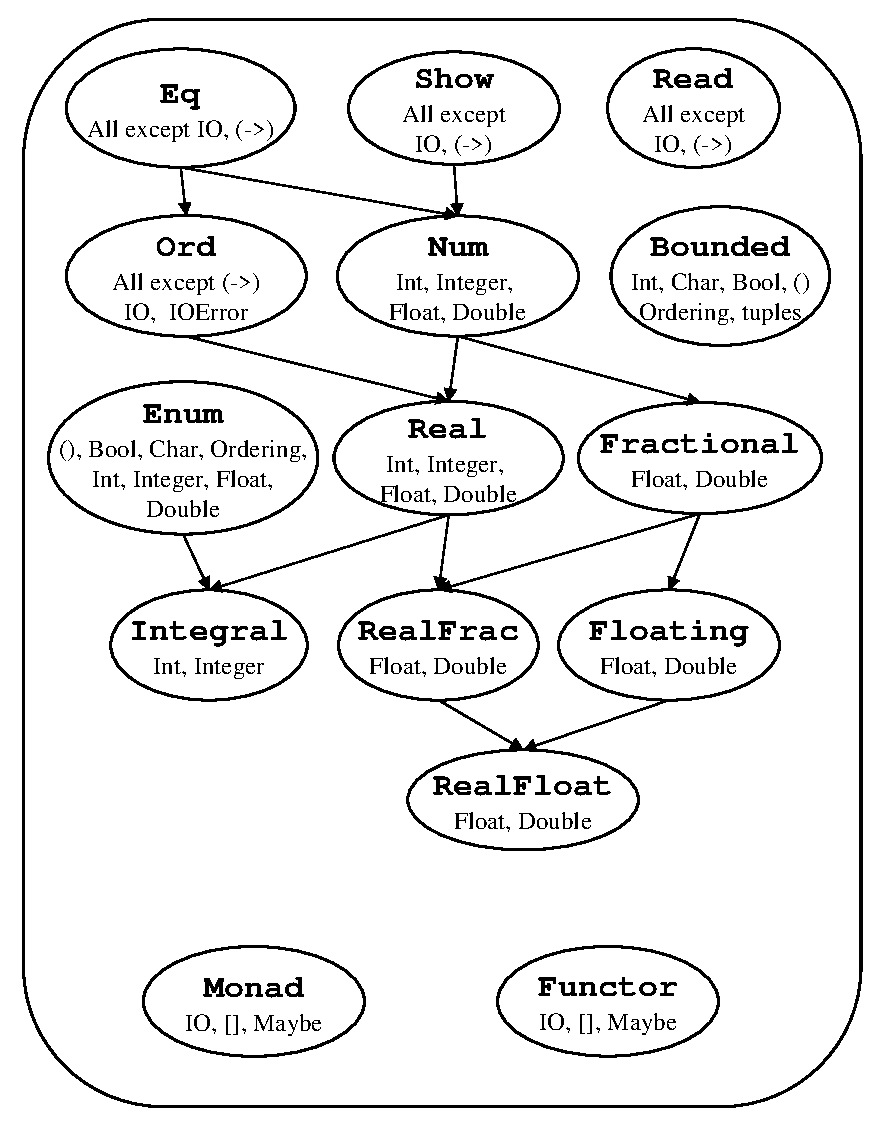
\includegraphics[scale=0.7]{classes}
% \struthack{11pt}
%*endignore
%**<div align=center><img src=\mbox{$\it classes.gif$} alt=\mbox{$\it Diagram\ of\ standard\ Haskell\ classes$}> 
%**<h4>Figure 5</h4> </div>
\ecaption{Standard Haskell Classes}
\label{standard-classes}
\end{figure}

Default class method declarations (Section~\ref{classes}) are provided
for many of the methods in standard classes.  A comment with each
\mbox{\tt class} declaration in Chapter~\ref{stdprelude} specifies the
smallest collection of method definitions that, together with the
default declarations, provide a reasonable definition for all the
class methods.  If there is no such comment, then all class methods
must be given to fully specify an instance.

\subsection{The Eq Class}
\indexclass{Eq}
\indextt{==}
\indextt{/=}
\bprog
{\small\begin{verbatim}
  class  Eq a  where
        (==), (/=)  ::  a -> a -> Bool

        x /= y  = not (x == y)
        x == y  = not (x /= y)
\end{verbatim}}
\eprog
The \mbox{\tt Eq} class provides equality (\mbox{\tt ==}) and inequality (\mbox{\tt /=}) methods.
All basic datatypes except for functions and \mbox{\tt IO} are instances of this class.
Instances of \mbox{\tt Eq} can be derived for any user-defined datatype whose
constituents are also instances of \mbox{\tt Eq}.

This declaration gives default method declarations for both \mbox{\tt /=} and \mbox{\tt ==},
each being defined in terms of the other.  If an instance declaration
for \mbox{\tt Eq} defines neither \mbox{\tt ==} nor \mbox{\tt /=}, then both will loop.
If one is defined, the default method for the other will make use of
the one that is defined.  If both are defined, neither default method is used.

\subsection{The Ord Class}
\indexclass{Ord}
\indextt{<}
\indextt{<=}
\indextt{>}
\indextt{>=}
\indextt{compare}
\indextt{max}
\indextt{min}
\bprog
{\small\begin{verbatim}
  class  (Eq a) => Ord a  where
    compare              :: a -> a -> Ordering
    (<), (<=), (>=), (>) :: a -> a -> Bool
    max, min             :: a -> a -> a

    compare x y | x == y    = EQ
                | x <= y    = LT
                | otherwise = GT

    x <= y  = compare x y /= GT
    x <  y  = compare x y == LT
    x >= y  = compare x y /= LT
    x >  y  = compare x y == GT

    -- Note that (min x y, max x y) = (x,y) or (y,x)
    max x y | x <= y    =  y
            | otherwise =  x
    min x y | x <= y    =  x
            | otherwise =  y
\end{verbatim}}
\eprog
The \mbox{\tt Ord} class is used for totally ordered datatypes.  All basic
datatypes
except for functions, \mbox{\tt IO}, and \mbox{\tt IOError}, are instances of this class.  Instances
of \mbox{\tt Ord} 
can be derived for any user-defined datatype whose constituent types
are in \mbox{\tt Ord}.  The declared order
of the constructors in the data declaration determines the ordering in
derived \mbox{\tt Ord} instances.
The \mbox{\tt Ordering} datatype
allows a single comparison to determine the precise ordering of two
objects.

The default declarations allow a user to create an \mbox{\tt Ord} instance 
either with a type-specific \mbox{\tt compare} function or with type-specific
\mbox{\tt ==} and \mbox{\tt <=} functions.

\subsection{The Read and Show Classes}
\indexsynonym{ReadS}
\indexsynonym{ShowS}
\indexclass{Read}
\indexclass{Show}
\indextt{show}
\indextt{readsPrec}
\indextt{showsPrec}
\indextt{readList}
\indextt{showList}
\bprog
{\small\begin{verbatim}
type  ReadS a = String -> [(a,String)]
type  ShowS   = String -> String

class  Read a  where
    readsPrec :: Int -> ReadS a
    readList  :: ReadS [a]
    -- ... default decl for readList given in Prelude

class  Show a  where
    showsPrec :: Int -> a -> ShowS
    show      :: a -> String 
    showList  :: [a] -> ShowS

    showsPrec _ x s   = show x ++ s
    show x            = showsPrec 0 x ""
    -- ... default decl for showList given in Prelude
\end{verbatim}}
\eprog
The \mbox{\tt Read} and \mbox{\tt Show} classes are used to convert values to
or from strings. 
The \mbox{\tt Int} argument to \mbox{\tt showsPrec} and \mbox{\tt readsPrec} gives the operator
precedence of the enclosing context (see Section~\ref{derived-text}).

\mbox{\tt showsPrec} and \mbox{\tt showList} return a \mbox{\tt String}-to-\mbox{\tt String}
function, to allow constant-time concatenation of its results using function
composition.
A specialised variant, \mbox{\tt show}, is also provided, which
uses precedence context zero, and returns an ordinary \mbox{\tt String}.
The method \mbox{\tt showList} is provided to allow the programmer to
give a specialised way of showing lists of values.  This is particularly
useful for the \mbox{\tt Char} type, where values of type \mbox{\tt String} should be
shown in double quotes, rather than between square brackets.

Derived instances of \mbox{\tt Read} and \mbox{\tt Show} replicate the style in which a
constructor is declared: infix constructors and field names are used
on input and output.  Strings produced by \mbox{\tt showsPrec} are usually
readable by \mbox{\tt readsPrec}.  

All \mbox{\tt Prelude} types, except function types and \mbox{\tt IO} types,
are instances of \mbox{\tt Show} and \mbox{\tt Read}.
(If desired, a programmer can easily make functions and \mbox{\tt IO} types 
into (vacuous) instances of \mbox{\tt Show}, by providing an instance declaration.)

\indextt{reads}
\indextt{shows}
\indextt{read}
For convenience, the Prelude provides the following auxiliary
functions: 
\bprog
{\small\begin{verbatim}
reads   :: (Read a) => ReadS a
reads   =  readsPrec 0

shows   :: (Show a) => a -> ShowS
shows   =  showsPrec 0

read    :: (Read a) => String -> a
read s  =  case [x | (x,t) <- reads s, ("","") <- lex t] of
              [x] -> x
              []  -> error "PreludeText.read: no parse"
              _   -> error "PreludeText.read: ambiguous parse"
\end{verbatim}}
\eprog
\indextt{shows}\indextt{reads}\indextt{show}\indextt{read}
\mbox{\tt shows} and \mbox{\tt reads} use a default precedence of 0.  The \mbox{\tt read} function reads
input from a string, which must be completely consumed by the input
process.  

\indextt{lex}
The function \mbox{\tt lex\ ::\ ReadS\ String}, used by \mbox{\tt read}, is also part of the Prelude.
It reads a single lexeme from the input, discarding initial white space, and
returning the characters that constitute the lexeme.  If the input string contains
only white space, \mbox{\tt lex} returns a single successful ``lexeme'' consisting of the
empty string.  (Thus \mbox{\tt lex\ ""} = \mbox{\tt [("","")]}.)  If there is no legal lexeme at the
beginning of the input string, \mbox{\tt lex} fails (i.e. returns \mbox{\tt []}).


\subsection{The Enum Class}
\label{enum-class}
\indexclass{Enum}
\indextt{toEnum}
\indextt{fromEnum}
\indextt{enumFrom}
\indextt{enumFromThen}
\indextt{enumFromTo}
\indextt{enumFromThenTo}
\bprog
{\small\begin{verbatim}
class  Enum a  where
    succ, pred     :: a -> a
    toEnum         :: Int -> a
    fromEnum       :: a -> Int
    enumFrom       :: a -> [a]            -- [n..]
    enumFromThen   :: a -> a -> [a]       -- [n,n'..]
    enumFromTo     :: a -> a -> [a]       -- [n..m]
    enumFromThenTo :: a -> a -> a -> [a]  -- [n,n'..m]

    -- Default declarations given in Prelude
\end{verbatim}}
\eprog
Class \mbox{\tt Enum} defines operations on sequentially ordered types.
The functions \mbox{\tt succ} and \mbox{\tt pred} return the successor and predecessor,
respectively, of a value.
The functions \mbox{\tt fromEnum} and \mbox{\tt toEnum} map values from a type in
\mbox{\tt Enum} to and from \mbox{\tt Int}.  
The \mbox{\tt enumFrom}... methods are used when translating arithmetic
sequences (Section~\ref{arithmetic-sequences}).

Instances of \mbox{\tt Enum} may be derived for any enumeration type (types
whose constructors have no fields); see Chapter~\ref{derived-appendix}.

For any type that is an instance of class \mbox{\tt Bounded} as well as \mbox{\tt Enum}, the following
should hold:
\begin{itemize}
\item The calls \mbox{\tt succ\ maxBound} and \mbox{\tt pred\ minBound} should result in
a runtime error.

\item \mbox{\tt fromEnum} and \mbox{\tt toEnum} should give a runtime error if the 
result value is not representable in the result type.  For example,
\mbox{\tt toEnum\ 7\ ::\ Bool} is an error.

\item \mbox{\tt enumFrom} and \mbox{\tt enumFromThen} should be defined with 
an implicit bound, thus:
\bprog
{\small\begin{verbatim}
  enumFrom     x   = enumFromTo     x maxBound
  enumFromThen x y = enumFromThenTo x y bound
    where
      bound | fromEnum y >= fromEnum x = maxBound
            | otherwise                = minBound
\end{verbatim}}
\eprog
\end{itemize}

The following \mbox{\tt Prelude} types are instances of \mbox{\tt Enum}: 
\begin{itemize}
\item Enumeration types: \mbox{\tt ()}, \mbox{\tt Bool}, and \mbox{\tt Ordering}. The
semantics of these instances is given by Chapter~\ref{derived-appendix}.
For example, \mbox{\tt [LT\ ..]} is the list \mbox{\tt [LT,EQ,GT]}.

\item \mbox{\tt Char}: the instance is given in Chapter~\ref{stdprelude}, based
on the primitive functions that convert between a \mbox{\tt Char} and an \mbox{\tt Int}.
For example, \mbox{\tt enumFromTo\ 'a'\ 'z'} denotes
the list of lowercase letters in alphabetical order.

\item Numeric types: \mbox{\tt Int}, \mbox{\tt Integer}, \mbox{\tt Float}, \mbox{\tt Double}.  The semantics
of these instances is given next.
\end{itemize}
For all four numeric types, \mbox{\tt succ} adds 1, and \mbox{\tt pred} subtracts 1.
The conversions \mbox{\tt fromEnum} and \mbox{\tt toEnum} convert between the type and \mbox{\tt Int}.
In the case of \mbox{\tt Float} and \mbox{\tt Double}, the digits after the decimal point may be lost.
It is implementation-dependent what \mbox{\tt fromEnum} returns when applied to 
a value that is too large to fit in an \mbox{\tt Int}.

For the types \mbox{\tt Int} and \mbox{\tt Integer}, the enumeration functions 
have the following meaning:
\begin{itemize}
\item The sequence \mbox{$\it \makebox{\tt enumFrom}~e_1$} is the list \mbox{$\it \makebox{\tt [}e_1\makebox{\tt ,}e_1+1\makebox{\tt ,}e_1+2\makebox{\tt ,}\ldots \makebox{\tt ]}$}.

\item The sequence \mbox{$\it \makebox{\tt enumFromThen}~e_1~e_2$} is the list \mbox{$\it \makebox{\tt [}e_1\makebox{\tt ,}e_1+i\makebox{\tt ,}e_1+2i\makebox{\tt ,}\ldots \makebox{\tt ]}$},
where the increment, \mbox{$\it i$}, is \mbox{$\it e_2-e_1$}.  The increment may be zero or negative.
If the increment is zero, all the list elements are the same.

\item The sequence \mbox{$\it \makebox{\tt enumFromTo}~e_1~e_3$} is 
the list \mbox{$\it \makebox{\tt [}e_1\makebox{\tt ,}e_1+1\makebox{\tt ,}e_1+2\makebox{\tt ,}\ldots e_3\makebox{\tt ]}$}.
The list is empty if \mbox{$\it e_1\ >\ e_3$}.

\item The sequence \mbox{$\it \makebox{\tt enumFromThenTo}~e_1~e_2~e_3$} 
is the list \mbox{$\it \makebox{\tt [}e_1\makebox{\tt ,}e_1+i\makebox{\tt ,}e_1+2i\makebox{\tt ,}\ldots e_3\makebox{\tt ]}$},
where the increment, \mbox{$\it i$}, is \mbox{$\it e_2-e_1$}.  If the increment 
is positive or zero, the list terminates when the next element would
be greater than \mbox{$\it e_3$}; the list is empty if \mbox{$\it e_1\ >\ e_3$}.
If the increment is negative, the list terminates when the next element would
be less than \mbox{$\it e_3$}; the list is empty if \mbox{$\it e1\ <\ e_3$}.
\end{itemize}
For \mbox{\tt Float} and \mbox{\tt Double}, the semantics of the \mbox{\tt enumFrom} family is
given by the rules for \mbox{\tt Int} above, except that the list terminates
when the elements become greater than \mbox{$\it e_3+i/2$} for positive increment
\mbox{$\it i$}, or when they become less than \mbox{$\it e_3+i/2$} for negative \mbox{$\it i$}.

For all four of these Prelude numeric types, all of the \mbox{\tt enumFrom} 
family of functions are strict in all their arguments.

\subsection{The Functor Class}
\indexclass{Functor}
\indextt{fmap}
\index{functor}

\bprog
{\small\begin{verbatim}
class  Functor f  where
    fmap    :: (a -> b) -> f a -> f b
\end{verbatim}}
\eprog
The \mbox{\tt Functor}
class is used for types that can be mapped over.  Lists, \mbox{\tt IO}, and
\mbox{\tt Maybe} are in this class. 

Instances of \mbox{\tt Functor} should satisfy the following laws:
\[\ba{lcl}
\mbox{\tt fmap\ id}&=&\mbox{\tt id}\\
\mbox{\tt fmap\ (f\ .\ g)}&=&\mbox{\tt fmap\ f\ .\ fmap\ g}\\
\ea\]\ifhtml{\\}{}
All instances of \mbox{\tt Functor} defined in the Prelude satisfy these laws.


\subsection{The Monad Class}
\label{monad-class}
\indexclass{Monad}
\indextt{return}
\indextt{fail}
\indextt{>>}
\indextt{>>=}
\index{monad}
\bprog
{\small\begin{verbatim}
class  Monad m  where
    (>>=)   :: m a -> (a -> m b) -> m b
    (>>)    :: m a -> m b -> m b
    return  :: a -> m a
    fail    :: String -> m a

    m >> k  =  m >>= \_ -> k
    fail s  = error s
\end{verbatim}}
\eprog
The \mbox{\tt Monad} class defines the basic operations over a {\em monad}.
See Chapter~\ref{io} for more information about monads.

``\mbox{\tt do}'' expressions provide a convenient syntax for writing
monadic expressions (see Section~\ref{do-expressions}).
The \mbox{\tt fail} method is invoked on pattern-match failure in a \mbox{\tt do}
expression.

In the Prelude, lists, 
\mbox{\tt Maybe}, and \mbox{\tt IO} are all instances of \mbox{\tt Monad}.
The \mbox{\tt fail} method for lists returns the empty list \mbox{\tt []},
for \mbox{\tt Maybe} returns \mbox{\tt Nothing}, and for \mbox{\tt IO} raises a user
exception in the IO monad (see Section~\ref{io-exceptions}).

Instances of \mbox{\tt Monad} should satisfy the following laws:
\[\ba{lcl}
\mbox{\tt return\ a\ >>=\ k}&=&\mbox{\tt k\ a} \\
\mbox{\tt m\ >>=\ return}&=&\mbox{\tt m} \\
\mbox{\tt m\ >>=\ ({\char'134}x\ ->\ k\ x\ >>=\ h)}&=&\mbox{\tt (m\ >>=\ k)\ >>=\ h}\\
\ea\]\ifhtml{\\}{}
Instances of both \mbox{\tt Monad} and \mbox{\tt Functor} should additionally satisfy the law:
\[\ba{lcl}
\mbox{\tt fmap\ f\ xs}&=&\mbox{\tt xs\ >>=\ return\ .\ f}\\
\ea\]\ifhtml{\\}{}
All instances of \mbox{\tt Monad} defined in the Prelude satisfy these laws.

The Prelude provides the following auxiliary functions: 
\bprog
{\small\begin{verbatim}
sequence  :: Monad m => [m a] -> m [a] 
sequence_ :: Monad m => [m a] -> m () 
mapM      :: Monad m => (a -> m b) -> [a] -> m [b]
mapM_     :: Monad m => (a -> m b) -> [a] -> m ()
(=<<)     :: Monad m => (a -> m b) -> m a -> m b
\end{verbatim}}
\eprog
\indextt{sequence}
\index{sequence{\char '137}@{\tt  sequence{\char '137}}}
\index{mapM{\char '137}@{\tt  mapM{\char '137}}}
\indextt{mapM}
\indextt{=<<}

\subsection{The Bounded Class}
\indexclass{Bounded}
\indextt{minBound}
\indextt{maxBound}
{\small\begin{verbatim}
class  Bounded a  where
    minBound, maxBound :: a
\end{verbatim}}

The \mbox{\tt Bounded} class is used to name the upper and lower limits of a
type.  \mbox{\tt Ord} is not a superclass of \mbox{\tt Bounded} since types that are not
totally ordered may also have upper and lower bounds.
The types \mbox{\tt Int}, \mbox{\tt Char}, \mbox{\tt Bool},
\mbox{\tt ()}, \mbox{\tt Ordering}, and all tuples are instances of \mbox{\tt Bounded}.  
The \mbox{\tt Bounded} class may be derived
for any enumeration type; \mbox{\tt minBound} is the first constructor listed
in the \mbox{\tt data} declaration and \mbox{\tt maxBound} is the last.  \mbox{\tt Bounded} may
also be derived for single-constructor datatypes whose constituent
types are in \mbox{\tt Bounded}.

\section{Numbers}
\label{numbers}
\index{number}

\Haskell{} provides several kinds of numbers; the numeric
types and the operations upon them have been heavily influenced by
%Common Lisp \cite{steele:common-lisp} and Scheme \cite{RRRRS}.
Common Lisp and Scheme.
Numeric function names and operators are usually overloaded, using
several type classes with an inclusion relation shown in
Figure~\ref{standard-classes}.
The class \mbox{\tt Num}\indexclass{Num} of numeric
types is a subclass of \mbox{\tt Eq}\indexclass{Eq}, since all numbers may be
compared for equality; its subclass \mbox{\tt Real}\indexclass{Real} is also a
subclass of \mbox{\tt Ord}\indexclass{Ord}, since the other comparison operations
apply to all but complex numbers (defined in the \mbox{\tt Complex} library).
The class \mbox{\tt Integral}\indexclass{Integral} contains integers of both 
limited and unlimited range; the class
\mbox{\tt Fractional}\indexclass{Fractional} contains all non-integral types; and
the class \mbox{\tt Floating}\indexclass{Floating} contains all floating-point
types, both real and complex.

The Prelude defines only the most basic numeric types: fixed sized
integers (\mbox{\tt Int}), arbitrary precision integers (\mbox{\tt Integer}), single
precision floating (\mbox{\tt Float}), and double precision floating
(\mbox{\tt Double}).  Other numeric types such as rationals and complex numbers
are defined in libraries.  In particular, the type \mbox{\tt Rational} is a
ratio of two \mbox{\tt Integer} values, as defined in the \mbox{\tt Ratio}
library.  

The default floating point operations defined by the \Haskell{}
Prelude do not 
conform to current language independent arithmetic (LIA) standards.  These
standards require considerably more complexity in the numeric
structure and have thus been relegated to a library.  Some, but not
all, aspects of the IEEE floating point standard have been
accounted for in Prelude class \mbox{\tt RealFloat}.

The standard numeric types are listed in Table~\ref{standard-numeric-types}.
The finite-precision integer type \mbox{\tt Int}\indextycon{Int} covers at
least the range 
\mbox{$\it [\ -\ 2^{29},\ 2^{29}\ -\ 1]\/$}.  As \mbox{\tt Int} is an instance of the \mbox{\tt Bounded}
class, \mbox{\tt maxBound} and \mbox{\tt minBound} can be used to determine the exact
\mbox{\tt Int} range defined by an implementation.
%(Figure~\ref{basic-numeric-2}, page~\pageref{basic-numeric-2}) define the limits of
%\mbox{\tt Int}\indextycon{Int} in each implementation.
\mbox{\tt Float}\indextycon{Float} is implementation-defined; it is desirable that
this type be at least equal in range and precision to the IEEE
single-precision type.  Similarly, \mbox{\tt Double}\indextycon{Double} should
cover IEEE double-precision.  The results of exceptional
conditions (such as overflow or underflow) on the fixed-precision
numeric types are undefined; an implementation may choose error
(\mbox{$\it \bot$}, semantically), a truncated value, or a special value such as
infinity, indefinite, etc.

\begin{table}[tb]
\[
\bto{|l|l|l|}
\hline
\multicolumn{1}{|c|}{Type} & 
        \multicolumn{1}{c|}{Class} &
        \multicolumn{1}{c|}{Description} \\ \hline
\mbox{\tt Integer} & \mbox{\tt Integral} & Arbitrary-precision integers \\
\mbox{\tt Int} & \mbox{\tt Integral} & Fixed-precision integers \\
\mbox{\tt (Integral\ a)\ =>\ Ratio\ a} & \mbox{\tt RealFrac} & Rational numbers \\
\mbox{\tt Float} & \mbox{\tt RealFloat} & Real floating-point, single precision \\
\mbox{\tt Double} & \mbox{\tt RealFloat} & Real floating-point, double precision \\
\mbox{\tt (RealFloat\ a)\ =>\ Complex\ a} & \mbox{\tt Floating} & Complex floating-point \\
\hline
\eto
\]
%**<div align=center> <h4>Table 2</h4> </div>
\ecaption{Standard Numeric Types}
\label{standard-numeric-types}
\index{numeric type}
\end{table}

The standard numeric classes and other numeric functions defined in
the Prelude are shown
in Figures~\ref{basic-numeric-1}--\ref{basic-numeric-2}.
Figure~\ref{standard-classes} shows the class dependencies and
built-in types that are instances of the numeric classes.

\begin{figure}[tb]
\begin{outlineenv}
{\small\begin{verbatim}
class  (Eq a, Show a) => Num a  where
    (+), (-), (*)  :: a -> a -> a
    negate         :: a -> a
    abs, signum    :: a -> a
    fromInteger    :: Integer -> a

class  (Num a, Ord a) => Real a  where
    toRational ::  a -> Rational

class  (Real a, Enum a) => Integral a  where
    quot, rem, div, mod :: a -> a -> a
    quotRem, divMod     :: a -> a -> (a,a)
    toInteger           :: a -> Integer

class  (Num a) => Fractional a  where
    (/)          :: a -> a -> a
    recip        :: a -> a
    fromRational :: Rational -> a

class  (Fractional a) => Floating a  where
    pi                  :: a
    exp, log, sqrt      :: a -> a
    (**), logBase       :: a -> a -> a
    sin, cos, tan       :: a -> a
    asin, acos, atan    :: a -> a
    sinh, cosh, tanh    :: a -> a
    asinh, acosh, atanh :: a -> a
\end{verbatim}}
\end{outlineenv}
%**<div align=center> <h4>Figure 6</h4> </div>
\ecaption{Standard Numeric Classes and Related Operations, Part 1}
\label{basic-numeric-1}
\indexclass{Num}
\indextt{+}
\indextt{-}
\indextt{*}
\indextt{negate}\indextt{abs}\indextt{signum}         
\indextt{fromInteger}
\indexclass{Real}\indextt{toRational}
\indexclass{Integral}
\indextt{quotRem}\indextt{divMod}\indextt{mod}\indextt{div}
\indextt{rem}\indextt{quot}
\indextt{even}\indextt{odd}
\indexclass{Fractional}
\indextt{/}
\indextt{recip}\indextt{fromRational}       
\indexclass{Floating}\indextt{pi}\indextt{exp}\indextt{log}\indextt{sqrt} 
\indextt{**}
\indextt{logBase}
\indextt{sin}\indextt{cos}\indextt{tan}                        
\indextt{asin}\indextt{acos}\indextt{atan}               
\indextt{sinh}\indextt{cosh}\indextt{tanh}               
\indextt{asinh}\indextt{acosh}\indextt{atanh}      
\end{figure}

\begin{figure}[tb]
\begin{outlineenv}
{\small\begin{verbatim}
class  (Real a, Fractional a) => RealFrac a  where
    properFraction   :: (Integral b) => a -> (b,a)
    truncate, round  :: (Integral b) => a -> b
    ceiling, floor   :: (Integral b) => a -> b

class  (RealFrac a, Floating a) => RealFloat a  where
    floatRadix          :: a -> Integer
    floatDigits         :: a -> Int
    floatRange          :: a -> (Int,Int)
    decodeFloat         :: a -> (Integer,Int)
    encodeFloat         :: Integer -> Int -> a
    exponent            :: a -> Int
    significand         :: a -> a
    scaleFloat          :: Int -> a -> a
    isNaN, isInfinite, isDenormalized, isNegativeZero, isIEEE 
                        :: a -> Bool
    atan2               :: a -> a -> a

gcd, lcm :: (Integral a) => a -> a-> a
(^)      :: (Num a, Integral b) => a -> b -> a
(^^)     :: (Fractional a, Integral b) => a -> b -> a

fromIntegral :: (Integral a, Num b) => a -> b
realToFrac   :: (Real a, Fractional b) => a -> b
\end{verbatim}}
\end{outlineenv}
%**<div align=center> <h4>Figure 7</h4> </div>
\ecaption{Standard Numeric Classes and Related Operations, Part 2}
\label{basic-numeric-2}
\indexclass{RealFrac}\indextt{properFraction}\indextt{approxRational}
\indextt{truncate}\indextt{round}
\indextt{ceiling}\indextt{floor}    
\indexclass{RealFloat}
\indextt{floatRadix}\indextt{floatDigits}\indextt{floatRange} 
\indextt{decodeFloat}\indextt{encodeFloat}
\indextt{exponent}\indextt{significand}\indextt{scaleFloat}
\indextycon{Int}\indextycon{Integer}
\indextt{fromIntegral}
\indextt{gcd}\indextt{lcm} 
\index{^@{\tt  {\char'136}}} % this is ^.  Must have 2 spaces after tt!
\index{^^@{\tt  {\char'136}{\char'136}}} % this is ^^
\indexclass{RealFrac}
\indextycon{Float}\indextycon{Double}
\indextt{realToFrac}
\indextt{atan2}
\end{figure}

\subsection{Numeric Literals}
\label{numeric-literals}

The syntax of numeric literals is given in
Section~\ref{lexemes-numeric}.  An integer literal represents the
application
of the function \mbox{\tt fromInteger}\indextt{fromInteger} to the appropriate
value of type 
\mbox{\tt Integer}.  Similarly, a floating literal stands for an application of
\mbox{\tt fromRational}\indextt{fromRational} to a value of type \mbox{\tt Rational} (that is, 
\mbox{\tt Ratio\ Integer}).  Given the typings:
\bprog
{\small\begin{verbatim}
fromInteger  :: (Num a) => Integer -> a
fromRational :: (Fractional a) => Rational -> a
\end{verbatim}}
\eprog\indextt{fromInteger}\indextt{fromRational}%
integer and floating literals have the
typings \mbox{\tt (Num\ a)\ =>\ a} and \mbox{\tt (Fractional\ a)\ =>\ a}, respectively.
Numeric literals are defined in this indirect way so that they may be
interpreted as values of any appropriate numeric type.
See Section~\ref{default-decls} for a discussion of overloading ambiguity.

\subsection{Arithmetic and Number-Theoretic Operations}
\label{arithmetic-operators}
\index{arithmetic operator}

The infix class methods 
\mbox{\tt (+)},
\indextt{+}
\mbox{\tt (*)},
\indextt{*}
\mbox{\tt (-)},
\indextt{-}
and the unary function
\mbox{\tt negate}\indextt{negate} (which can also be written as a prefix minus sign; see
section~\ref{operators}) apply to all numbers.  The class methods
\mbox{\tt quot}\indextt{quot}, \mbox{\tt rem}\indextt{rem}, \mbox{\tt div}\indextt{div}, and
\mbox{\tt mod}\indextt{mod} apply only to integral numbers, while the class method
\mbox{\tt (/)}
\indextt{/}
applies only to fractional ones.  The \mbox{\tt quot}, \mbox{\tt rem},
\mbox{\tt div}, and \mbox{\tt mod} class methods satisfy these laws if \mbox{\tt y} is non-zero:
\bprog
{\small\begin{verbatim}
(x `quot` y)*y + (x `rem` y) == x
(x `div`  y)*y + (x `mod` y) == x
\end{verbatim}}
\eprog
\mbox{\tt `quot`} is integer division truncated toward zero,
while the result of \mbox{\tt `div`} is truncated toward
negative infinity. 
%Note that \mbox{\tt quot} should be used rather than
%\mbox{\tt div} to give the semantics of Pascal's \mbox{\tt div}.
The \mbox{\tt quotRem} class method takes a dividend and a divisor as arguments
and returns a (quotient, remainder) pair; \mbox{\tt divMod} is defined
similarly:
\bprog
{\small\begin{verbatim}
quotRem x y  =  (x `quot` y, x `rem` y)
divMod  x y  =  (x `div`  y, x `mod` y)
\end{verbatim}}
\eprog
Also available on integral numbers are the even and odd predicates:
\bprog
{\small\begin{verbatim}
even x =  x `rem` 2 == 0
odd    =  not . even
\end{verbatim}}
\eprog\indextt{even}\indextt{odd}
Finally, there are the greatest common divisor and least common
multiple functions.  \mbox{\tt gcd}\indextt{gcd} \mbox{$\it x$} \mbox{$\it y$} is the greatest
(positive) integer that divides both \mbox{$\it x$} and \mbox{$\it y$}; for example \mbox{\tt gcd\ (-3)\ 6} = \mbox{\tt 3}, \mbox{\tt gcd\ (-3)\ (-6)} = \mbox{\tt 3}, 
\mbox{\tt gcd\ 0\ 4} = \mbox{\tt 4}. \mbox{\tt gcd\ 0\ 0} raises a runtime error.

\mbox{\tt lcm}\indextt{lcm} \mbox{$\it x$} \mbox{$\it y$} is the smallest positive integer that both \mbox{$\it x$} and \mbox{$\it y$} divide.

\subsection{Exponentiation and Logarithms}
\index{exponentiation}\index{logarithm}

The one-argument exponential function \mbox{\tt exp}\indextt{exp} and the
logarithm function \mbox{\tt log}\indextt{log} act on floating-point numbers and
use base \mbox{$\it e$}.  \mbox{\tt logBase}\indextt{logBase} \mbox{$\it a$} \mbox{$\it x$} returns the
logarithm of \mbox{$\it x$} in base \mbox{$\it a$}.  \mbox{\tt sqrt}\indextt{sqrt} returns the
principal square root of a floating-point number.
There are three two-argument exponentiation operations:
\mbox{\tt ({\char'136})}\index{^@{\tt  {\char'136}}} raises any  % 
number to a nonnegative integer power,
\mbox{\tt ({\char'136}{\char'136})}\index{^^@{\tt  {\char'136}{\char'136}}} raises a
fractional number to any integer power, and \mbox{\tt (**)}
\indextt{**}
takes two floating-point arguments.  The value of \mbox{$\it x$}\mbox{\tt {\char'136}0} or \mbox{$\it x$}\mbox{\tt {\char'136}{\char'136}0}
is \mbox{\tt 1} for any \mbox{$\it x$}, including zero; \mbox{\tt 0**}\mbox{$\it y$} is \mbox{\tt 1} if \mbox{$\it y$} is \mbox{\tt 0}, and
\mbox{\tt 0} otherwise.
  
\subsection{Magnitude and Sign}
\label{magnitude-sign}
\index{magnitude}\index{sign}

A number has a {\em magnitude}
and a {\em sign}.  The functions \mbox{\tt abs}\indextt{abs} and
\mbox{\tt signum}\indextt{signum} apply to any number and satisfy the law:
\bprog
{\small\begin{verbatim}
abs x * signum x == x
\end{verbatim}}
\eprog
For real numbers, these functions are defined by:
\bprog
{\small\begin{verbatim}
abs x    | x >= 0  = x
         | x <  0  = -x

signum x | x >  0  = 1
         | x == 0  = 0
         | x <  0  = -1
\end{verbatim}}
\eprog

\subsection{Trigonometric Functions}
\index{trigonometric function}

Class \mbox{\tt Floating} provides the 
circular and hyperbolic sine\index{sine}, cosine\index{cosine},
and tangent\index{tangent} functions and their inverses.
Default implementations of \mbox{\tt tan}, \mbox{\tt tanh}, \mbox{\tt logBase}, \mbox{\tt **}, and \mbox{\tt sqrt} are
provided, but implementors are free to provide more accurate implementations.

Class \mbox{\tt RealFloat} provides a version of arctangent
taking two real floating-point arguments.
For real floating \mbox{$\it x$} and \mbox{$\it y$}, \mbox{\tt atan2}\indextt{atan2} \mbox{$\it y$} \mbox{$\it x$}
computes the angle (from the positive x-axis) of the vector from the origin
to the point \mbox{$\it (x,y)$}.  \mbox{\tt atan2}\indextt{atan2} \mbox{$\it y$} \mbox{$\it x$}
returns a value in the range \mbox{\tt [-pi,\ pi]}.  It
follows the Common Lisp semantics for the origin when signed zeroes are
supported.  \mbox{\tt atan2} \mbox{$\it y$} \mbox{\tt 1}, with \mbox{$\it y$} in a type that is \mbox{\tt RealFloat}, should return the
same value as \mbox{\tt atan} \mbox{$\it y$}.  A default definition of \mbox{\tt atan2} is provided, but
implementors can provide a more accurate implementation. 

The precise definition of the above functions is as in Common Lisp,
which in turn follows Penfield's proposal for
APL~\cite{penfield:complex-apl}.  See these references for discussions
of branch cuts, discontinuities, and implementation.

\subsection{Coercions and Component Extraction}
\label{coercion}
\index{coercion}

The \mbox{\tt ceiling}\indextt{ceiling}, \mbox{\tt floor}\indextt{floor},
\mbox{\tt truncate}\indextt{truncate}, and \mbox{\tt round}\indextt{round}
functions each take a real fractional argument and return an integral
result.  \mbox{\mbox{\tt ceiling} \mbox{$\it x$}} returns the least integer not less than \mbox{$\it x$}, and
\mbox{\mbox{\tt floor} \mbox{$\it x$}}, the greatest integer not greater than \mbox{$\it x$}.  \mbox{\mbox{\tt truncate} \mbox{$\it x$}}
yields the integer nearest \mbox{$\it x$} between \mbox{$\it 0$} and \mbox{$\it x$}, inclusive.
\mbox{\mbox{\tt round} \mbox{$\it x$}} returns the nearest integer to \mbox{$\it x$}, the even integer if
\mbox{$\it x$} is equidistant between two integers.

%       Keith Wansbrough clarifies the above defn of \mbox{\tt round},
%       which strangely rounds both 3.5 and 4.5 to 4
%
% This is generally considered the most accurate kind of rounding, since it 
% avoids cumulative errors.  If you get lots of values on the 0.5 boundary, 
% `round up' gives you an error of +0.5 for each, whereas round-to-even gives 
% you a mean error of zero.
% 
% IEEE floating point does this by default for its basic operations.

The function \mbox{\tt properFraction}\indextt{properFraction} takes a real
fractional number \mbox{$\it x$} and returns a pair \mbox{$\it (n,f)$} such that \mbox{$\it x\ =\ n+f$}, and:
\mbox{$\it n$} is an integral number with the same sign as \mbox{$\it x$}; and \mbox{$\it f$} is a
fraction \mbox{$\it f$} with the same type and sign as \mbox{$\it x$}, and with absolute
value less than 1.
The \mbox{\tt ceiling}, \mbox{\tt floor}, \mbox{\tt truncate}, and \mbox{\tt round}
functions can be defined in terms of \mbox{\tt properFraction}.

Two functions convert numbers to type \mbox{\tt Rational}:
\mbox{\tt toRational}\indextt{toRational} returns the rational equivalent of
its real argument with full precision;
\mbox{\tt approxRational}\indextt{approxRational} takes two real fractional arguments
\mbox{$\it x$} and \mbox{$\it \epsilon$} and returns the simplest rational number within
\mbox{$\it \epsilon$} of \mbox{$\it x$}, where a rational $ p/q $ in reduced form is
{\em simpler} than another $ p^{\prime} / q^{\prime} $ if 
$ |p| \leq |p^{\prime}| $ and $ q \leq q^{\prime} $.
Every real interval contains a unique simplest rational;
in particular, note that $ 0/1 $ is the simplest rational of all.%
%\cite[Section 6.5.5]{RRRRS}.

The class methods of class \mbox{\tt RealFloat}\indexclass{RealFloat} allow
efficient, machine-independent
access to the components of a floating-point number.
The functions \mbox{\tt floatRadix}\indextt{floatRadix},
\mbox{\tt floatDigits}\indextt{floatDigits}, and
\mbox{\tt floatRange}\indextt{floatRange} give the parameters of a
floating-point type:  the radix of the representation, the number of
digits of this radix in the significand, and the lowest and highest
values the exponent may assume, respectively.
The function \mbox{\tt decodeFloat}\indextt{decodeFloat}
applied to a real floating-point number returns the significand
expressed as an \mbox{\tt Integer} and an appropriately scaled exponent (an
\mbox{\tt Int}).  If \mbox{\mbox{\tt decodeFloat\ x}} yields \mbox{\mbox{\tt (}\mbox{$\it m$}\mbox{\tt ,}\mbox{$\it n$}\mbox{\tt )}}, then \mbox{\tt x} is
equal in value to \mbox{$\it mb^n$}, where \mbox{$\it b$} is the floating-point radix, and
furthermore, either \mbox{$\it m$} and \mbox{$\it n$} are both zero or else
\mbox{$\it b^{d-1}\leq |m|<b^d$}, where \mbox{$\it d$} is the value of \mbox{\mbox{\tt floatDigits\ x}}.
\mbox{\tt encodeFloat}\indextt{encodeFloat} performs the inverse of this
transformation.  The functions \mbox{\tt significand}\indextt{significand}
and \mbox{\tt exponent}\indextt{exponent} together provide the same
information as \mbox{\tt decodeFloat},  but rather than an \mbox{\tt Integer},
\mbox{\mbox{\tt significand\ x}} yields a value of the same type as \mbox{\tt x}, scaled to lie
in the open interval \mbox{$\it (-1,1)$}.  \mbox{\mbox{\tt exponent\ 0}} is zero.  \mbox{\tt scaleFloat}
multiplies a floating-point number by an integer power of the radix.

The functions \mbox{\tt isNaN}, \mbox{\tt isInfinite}, \mbox{\tt isDenormalized},
\mbox{\tt isNegativeZero}, and \mbox{\tt isIEEE} all support numbers represented using
the IEEE standard.  For non-IEEE floating point numbers, these may all
return false.

Also available are the following coercion functions:
\bprog
{\small\begin{verbatim}
fromIntegral :: (Integral a, Num b)    => a -> b
realToFrac   :: (Real a, Fractional b) => a -> b
\end{verbatim}}
\eprogNoSkip\indextt{fromIntegral}\indextt{realToFrac}


%**~footer

% Local Variables: 
% mode: latex
% End:
